Using General Relativity we were able to write down an expression for the strain induced in an interferometer from a passing gravitational wave. In this chapter we provide a survey of how to detect gravitational-wave signals from \acp{CBC} in the interferometer data in the presence of noise. We begin by deriving the \emph{matched filter} for a single template, which is the optimal filter if the detector noise is stationary and Gaussian. Next, we show how matched filtering can be performed for a bank of templates in order to recover the parameters of a signal. This is followed by a discussion of the $\chi^2$ test, which can be used to suppress triggers from non-Gaussian transients that are present in real detector data. Finally, we describe how a coincidence test can be performed across multiple detectors to further decrease the number of false noise triggers produced by a search.

\section{Detecting a Gravitational Wave Using a Matched Filter}
\label{sec:matched_filter}

Equation \ref{eqn:GW_strain} gave the strain, $h(t)$, induced in an interferometer when a gravitational wave from an inspiraling compact binary with non-spinning component masses passes through. The strain was a function of chirp mass, $\mchirp$, and symmetric-mass ratio, $\eta$. If we wish to search for a gravitational wave that came from a binary with given $\mchirp$ and $\eta$, we can generate a waveform, or \emph{template}, that characterizes it. We now address the question: if a gravitational wave that matches our template exists in the \ac{IFO} data, how do we find it?

Let the output of the detector be the time series $s(t)$, which is a measure of the displacement of the \ac{IFO}'s mirrors as a function of time. If a gravitational wave with waveform $h(t)$ exists in the data, then:

\begin{equation}
\label{eqn:ifo_data}
s(t) = h(t) + n(t)
\end{equation}
where $n(t)$ is the strain induced by all other, non gravitational-wave,  sources, or ``noise," as a function of time. If no signal exists in the data, then $s(t) = n(t)$. We do not know \emph{a priori} if $h$ exists in the data; further, even if $h$ does exist, we do not know \emph{when} it occurs --- that is, we do not know its coalescence time, $\tau_c$.\footnote{Note that the exact time when $h$ occurs is somewhat arbitrary. We could choose any point in the evolution of the waveform and label that as the point that $h$ occurs. For \ac{CBC} templates, we chose to use the time of coalescence since it is easily identifiable: it is the point that the \ac{pN} approximation goes to infinite frequency.} Our goal, then, is to find a filter that takes $s(t)$ and $h(t-\tau)$ as input and returns a number, $\rho(\tau)$, that is proportional to the probability that $h$ is in $s$ with coalescence time $\tau$, $P(h(t-\tau)|s(t))$. We additionally require that, if $h$ is in $s$, this filter is at a maximum at the point that $h$ occurs. If we have such a filter --- known as the \emph{optimal filter} --- then we can determine that a signal exists in the data if $\rho(\tau)$ exceeds some pre-determined threshold $\rho^{*}$. Further, we can determine the coalescence time of $h$ by simply incrementing $\tau$ and evaluating $\rho$ at each increment, selecting points when $\rho$ is at a maximum. (This is known as the method of maximum likelihood \cite{Brown}.)

We begin by assuming that $\tau = \tau_c = 0$ and looking for the filter that maximizes $P(h|s)$ (for now, we will drop the ``$(t)$" for clarity). The problem of finding an optimal filter to extract signals from (Gaussian) noise is well studied, and has been applied to radar analysis for decades. Here, we follow the method outlined in \cite{Finn1992,FinnChernoff:1993,Brown} --- all of which use methods detailed in Wanstein and Zubakov \cite{wainstein:1962} --- to derive the filter.

Using Bayes' theorem \cite{Sivia:DataAnalysis:2E} we can write $P(h|s)$ as:
\begin{equation}
\label{eqn:P_of_h1}
P(h|s) = \frac{P(s|h) P(h)}{P(s)}
\end{equation}
where:
\begin{eqnarray}
P(s|h) & \equiv & \mbox{the probability of getting $s$ if $h$ exists in it} \nonumber \\
P(h)   & \equiv & \mbox{the probability of the signal, $h$, occurring} \nonumber \\
P(s)   & \equiv & \mbox{the probability of getting $s$} \nonumber
\end{eqnarray}
Since the signal either does or does not exist in the data, the probability of getting a particular instance of $s$ is:
\begin{equation}
P(s) = P(s|0)P(0) + P(s|h)P(h)
\end{equation}
where:
\begin{eqnarray}
P(s|0) & \equiv & \mbox{the probability of getting $s$ if no signal exists} \nonumber \\
P(0) & \equiv & \mbox{the probability of getting no signal} \nonumber
\end{eqnarray}
Substituting this into \ref{eqn:P_of_h1} we have:
\begin{eqnarray}
\label{eqn:P_of_h}
P(s|h) & = & \frac{ P(s|h) P(h) }{ P(s|0)P(0) + P(s|h)P(h) } \nonumber \\
 & = & \frac{ P(s|h) } { P(s|0) \left(\, P(0)/P(h) + P(s|h)/P(s|0) \,\right) } \nonumber \\
 & = & \frac{ \Lambda }{ P(0)/P(h) + \Lambda }
\end{eqnarray}
where
\begin{equation}
\label{eqn:likelihood_ratio}
\Lambda \equiv \frac{ P(s|h) }{ P(s|0) }
\end{equation}
is the \emph{likelihood ratio}. $P(0)$ and $P(h)$ are known as \emph{priors}: they represent our \emph{a priori} belief that a signal does or does not exist, irrespective of the detector's ability to detect it. We do not need to concern ourselves with assigning values to them, however. Instead we note that $P(s|h)$ is a monotonically increasing function of $\Lambda$. Therefore, since we are only interested in a filter that maximizes $P(s|h)$ --- and not the exact value of $P(s|h)$ --- we can limit our focus to evaluating $\Lambda$, and threshold on the point that it reaches a maximum. We further note that the natural logarithm of $\Lambda$ also increases monotonically with $P(s|h)$. Since we will be interested in evaluating the likelihood in the region that $\Lambda$ is a maximum, it is common practice to instead evaluate the \emph{log-likelihood}, $\ln \Lambda$, instead, as it varies less rapidly around the region of interest \cite{Sivia:DataAnalysis:2E}.

Before calculating the log-likelihood, we note that we do not know \emph{a priori} the phase of the binary, $\theta$. Therefore, we treat $\theta$ as a \emph{nuisance} parameter, which we marginalize over \cite{Sivia:DataAnalysis:2E}. Thus, we write the likelihood ratio as:
\begin{eqnarray}
\Lambda & = & \int_0^{2 \pi} p(\theta) \lambda(\theta) \d\theta \nonumber \\
 & = & \frac{1}{2\pi P(s|0)} \int_0^{2 \pi} p(s|h(\theta)) \d\theta
\end{eqnarray}
Here, $\lambda(\theta)$ is the likelihood ratio at a given $\theta$, $p(\theta)$ is the prior probability of getting $\theta$, and we have written $P(s|h)$ as the \ac{PDF} $p(s|h(\theta))$; $P(s|0)$ remains outside of the integral as it has no $\theta$ dependence. Assuming any phase is equally likely, we set $p(\theta) = 1/2\pi$ and pulled it out of the integral, also.

To calculate the likelihood ratio, we need $p(s|h(\theta))$ and $P(s|0)$. We focus first on $P(s|0)$. If $s(t)$ has no signal in it then it is simply $n(t)$. $P(s|0)$ is therefore the probability of getting a particular realization of the noise. Let us assume that the noise is a stationary Gaussian process with zero mean. For our purposes it will be useful to characterize the noise by its \ac{PSD} rather than its variance. The \ac{PSD} is defined as the Fourier Transform of the autocorrelation of the noise \cite{wainstein:1962}:
\begin{equation}
S_n(f) \equiv \int_{-\infty}^{\infty} R(\tau)e^{-i 2\pi ft} \d t = \overline{\widetilde{n}^{*}(f)\widetilde{n}(f)}
\end{equation}
where,
\begin{equation}
R(\tau) = \overline{n(t)n(t-\tau)}
\end{equation}
is the autocorrelation function. Note that $R(0) = \overline{n(t)^2}$, which is the variance since $\overline{n(t)} = 0$. We restrict our analysis to positive frequencies; thus we will use the one-sided \ac{PSD} $S_n(|f|) = S_n(f)/2$. It is shown in \cite{Finn1992} that with these assumptions, the probability of getting a given realization of the noise, $n = s$, is:
\begin{equation}
\label{eqn:p_no_sig}
P(s|0) = \alpha \exp[ - \frac{1}{2} (s|s) ]
\end{equation}
where $\alpha$ is a normalization constant and the inner-product $(\cdot|\cdot)$ is defined as:
\begin{eqnarray}
\label{eqn:inner_product1}
(a|b) & \equiv & \int_{-\infty}^{\infty} \frac{ \widetilde{a}^{*}(f)\widetilde{b}(f) + \widetilde{a}(f)\widetilde{b}^{*}(f) }{S_n(|f|)} \d f \\
\label{eqn:inner_product2}
 & = & 2 \int_{-\infty}^{\infty} \frac{ \widetilde{a}^{*}(f)\widetilde{b}(f) }{S_n(|f|)} \d f
\end{eqnarray}
In going from \ref{eqn:inner_product1} to \ref{eqn:inner_product2} we have used the fact that for real functions of time (which both $h$ and $s$ are), $\widetilde{g}^{*}(f) = \widetilde{g}(-f)$.

Using this result we can also find $p(s|h(\theta))$. If $h$ is in the data, then $n(t) = s(t) - h(t, \theta)$. Thus,
\begin{eqnarray}
\label{eqn:p_sig}
p(s|h) & = & \alpha \exp\{ -\frac{1}{2} (s - h | s - h ) \} \nonumber \\
 & = & \alpha \exp\{ -\frac{1}{2} [ (s|s) - 2(h|s) + (h|h) ] \} \nonumber \\
 & = & P(s|0) \exp\{ (h|s) - (h|h)/2 \}
\end{eqnarray}
Substituting \ref{eqn:p_no_sig} and \ref{eqn:p_sig} into \ref{eqn:likelihood_ratio}, the likelihood ratio becomes:
\begin{eqnarray}
\label{eqn:lambda1}
\Lambda & = & \frac{1}{2\pi} \int_0^{2\pi} \exp\{ (h|s)- \frac{(h|h)}{2} \} \d\theta \\
\label{eqn:lambda2}
 & = & \frac{1}{2\pi} e^{-(h|h)/2} \int_0^{2\pi} \exp\{ (~C(t)\cos(2\phi(t) - \theta)~|~s~) \} \d\theta
\end{eqnarray}
In going from \ref{eqn:lambda1} to \ref{eqn:lambda2} we have used the general form of $h(t,\theta)$ given in equation \ref{eqn:GW_strain}, with $C(t) = A(t)/\effD$. We have also pulled the $(h|h)$ term out of the integral as it is simply a number --- it is the inner product of $h$ with itself --- and has no phase dependence. In order to evaluate the integral, we re-write the inner product of $s$ with $h$ as follows:
\begin{eqnarray}
\label{eqn:sh_in_z}
(h|s) & = &  (~C(t) \cos(2\phi(t) - \theta)~|~s(t)~) \nonumber \\
 & = & (~C(t)\cos(2\phi(t))~|~s(t)~) \cos(\theta) + (~C(t)\sin(2\phi(t))~|~s(t)~) \sin(\theta) \nonumber \\
 & = & x \cos(\theta) + y\sin(\theta) \nonumber \\
 & = & |z|\cos(\Phi)\cos(\theta) + |z|\sin(\Phi)\sin(\theta) \nonumber \\
 & = & |z|\cos(\Phi - \theta)
\end{eqnarray}
where:
\begin{align}
\label{eqn:matchf_x}
x = (~C(t)\cos(2\phi(t))~|~s(t)~) \equiv (h_{\pls}|s) \\
\label{eqn:matchf_y}
y = (~C(t)\sin(2\phi(t))~|~s(t)~) \equiv (h_{\crs}|s) \\
|z| = \sqrt{ x^2 + y^2 } \\
\Phi =  \tan^{-1}\left( \frac{y}{x} \right) 
\end{align}
Since the \ac{GW} phase, $2\phi(t)$, is $90^{\circ}$ out of phase in equations \ref{eqn:matchf_x} and \ref{eqn:matchf_y}, we have identified $x$ and $y$ as the inner products of the plus and cross polarizations, respectively, with the data. Due to their orthogonality, note that:
\begin{align}
(h_\pls|h_\pls) &= (h_\crs|h_\crs) &= (h|h) \\
(h_\pls|h_\crs) &= (h_\crs|h_\pls) &= 0
\end{align}
Also note that we can let $z$ be complex:
\begin{equation}
\label{eqn:complex_z}
z = x + iy
\end{equation}
This will prove useful below.

%Note that in this case we can write:
%\begin{align*}
%z &= (h_c|s) + i(h_s|s) \\
%  &= (h_c|s) + (-ih_s|s) \\
%  &= (h_c - ih_s|s) \\
%  &= (H|s)
%\end{align*}
%where $H$ is the phasor:
%\begin{equation}
%H(t) = C(t)e^{-i2\phi(t)}
%\end{equation}
%
%Using this formalism we can write:
%\begin{align}
%\label{eqn:matchf_xcmplx}
%x &= \Re(h|s) \\
%\label{eqn:matchf_ycmplx}
%y &= \Re (ih|s) \\
%\label{eqn:matchf_cmplx}
%z &=  (h|s) + i(h|s) \\
%\Rightarrow |z| &= \sqrt{2} (h|s)
%\end{align}
%Here $\Re$ denotes the real part of the functions. Using this complex notation will prove useful below.

Substituting equation \ref{eqn:sh_in_z} into the likelihood ratio, we have:
\begin{eqnarray}
\Lambda & = & \frac{1}{2\pi} e^{-(h|h)/2} \int_0^{2\pi} \exp\{ |z|\cos(\Phi - \theta) \} \d \theta \nonumber \\
 & = & e^{-(h|h)/2} I_0(|z|) \nonumber \\
\label{eqn:modBessel}
 & = & e^{-(h|h)/2} \sum_{k=0}^{\infty} \frac{(|z|^{2}/4)^{k}}{(k!)^2} \\
 \label{eqn:posDef}
 & \leq & e^{-(h|h)/2} \left( \sum_{k=0}^{\infty} \frac{ (|z|^{2}/4)^k }{k!} \right) \left(\sum_{m=0}^{\infty} \frac{1}{m!}\right) \\
 & \leq & e^{-(h|h)/2} e^{|z|^{2}/4 - 1}
\end{eqnarray}
where $I_0(|z|)$ is the modified Bessel function of the first kind, which is equal to the sum in equation \ref{eqn:modBessel} \cite{Weisstein:ModBessel:Wolfram}. To go from equation \ref{eqn:modBessel} to \ref{eqn:posDef} we have used the fact that $(|z|^{2}/4)^{k}/k!$ and $1/k!$ are positive definite for all $k$. Thus, the likelihood ratio is maximized when it is equal to $\exp\{ |z|^2/4 + 1 - (h|h)/2 \}$, and so we can threshold when the log-likelihood is:
\begin{equation}
\ln \Lambda = \frac{1}{4}|z|^2 + 1 - \frac{1}{2}(h|h)
\end{equation}
The factor of $1/4$ and the $+1$ term on the right-hand side of the equation only scale and offset $\ln\Lambda$ by constants. We can therefore threshold on:
\begin{equation}
4 \ln \Lambda - 4 = |z|^2 - 2(h|h)
\end{equation}
instead, without any loss in ability to detect $h$. The $(h|h)$ term, however, causes the log-likelihood to be template dependent. Since we will be filtering multiple templates, we prefer to use a quantity that is independent of the template used. Therefore, we normalize both sides by $(h|h)$. Dropping the remaining $-2$ offset, we are left with:
\begin{equation}
\frac{|z|^2}{(h|h)} \equiv \rho^{2}
\end{equation}
The quantity $\rho^2$ is our detection statistic.

In the absence of a signal, $(h|h)$ is the variance of the filter. To see this, first note that the mean of $(h|n)$ is zero:
\begin{eqnarray}
\overline{(h|n)} & = & 2 \overline{\int_{-\infty}^{\infty} \frac{\widetilde{h}^{*}(f)\widetilde{n}(f)}{S_n(|f|)} \d f} \nonumber \\
 & = & 2 \int_{-\infty}^{\infty} \frac{\widetilde{h}^{*}(f)\overline{\widetilde{n}(f)}}{S_n(|f|)} \d f \nonumber \\
 & = & 0
\end{eqnarray}
since $\overline{n(t)} = \overline{\widetilde{n}(f)} = 0$. The mean of the square of $(h|n)$ is:
\begin{eqnarray}
\overline{(h|n)^2} & = & \overline{\left| 2 \int_{-\infty}^{\infty} \frac{\widetilde{h}^{*}(f)\widetilde{n}(f)}{S_n(|f|)} \d f \right|^2 } \nonumber \\
 & = & 4 \int_{-\infty}^{\infty} \int_{-\infty}^{\infty} \frac{\widetilde{h}(f')\widetilde{h}^{*}(f)\overline{\widetilde{n}^{*}(f')\widetilde{n}(f)}}{S_n(|f'|)S_n(|f|)} \d f' \d f \nonumber \\
 & = & 4 \int_{-\infty}^{\infty} \int_{-\infty}^{\infty} \frac{\widetilde{h}(f')\widetilde{h}^{*}(f) S_n(|f'|)\delta(f'-f)}{2 S_n(|f'|)S_n(|f|)} \d f' \d f \nonumber \\
 & = & 2 \int_{-\infty}^{\infty} \frac{\widetilde{h}(f)\widetilde{h}(f)}{S_n(|f|)} \d f \nonumber \\
 & = & (h|h)
\end{eqnarray}
Thus the variance is:
\begin{equation}
\sigma^2 = \overline{(h|n)^2} - \overline{(h|n)}^2 = (h|h)
\end{equation}
and we can write:
\begin{equation}
\label{eqn:SNR}
\rho^2 = \frac{|z|^2}{\sigma^2}
\end{equation}
We therefore identify $\rho$ as the \emph{\ac{SNR}} of the template.

In order to evaluate $\rho$ for arbitrary values of $\tau \neq \tau_c \neq 0$, we note that the Fourier Transform of $h(t-\tau)$ is: 
\begin{eqnarray}
\widetilde{h}(f) & = & \int_{-\infty}^{\infty} h(t-\tau) e^{-i 2\pi f t} \d t \nonumber \\
& = & e^{i 2\pi f \tau} \int_{-\infty}^{\infty} h(t') e^{-i 2\pi ft'} \d t' \nonumber \\
& = & e^{i 2\pi f \tau} \widetilde{h}(f')
\end{eqnarray}
$\widetilde{h}(f')$ is the Fourier Transform of $h(t)$ independent of the coalescence time. We can thereby account for the unknown coalescence time by filtering:
\begin{equation*}
e^{-i 2\pi f\tau} \widetilde{h}(f)
\end{equation*}
This introduces a time-dependence to $\rho$:
\begin{align}
\rho(\tau)^2 &= \frac{|z(\tau)|^2}{\sigma^2} \nonumber \\
 &= \frac{1}{\sigma^2}\left( (h_{\pls}(\tau)|s)^2 + (h_{\crs}(\tau)|s)^2 \right) \nonumber \\
\label{eqn:snr_full_form}
 &= \frac{1}{\sigma^2}\left\{ \left( \int_{-\infty}^{\infty} \frac{\widetilde{h}_{\pls}^{*}(f)\widetilde{s}(f)}{S_n(|f|)} e^{i 2\pi f\tau} \d f \right)^2 + \left( \int_{-\infty}^{\infty} \frac{\widetilde{h}_{\crs}^{*}(f)\widetilde{s}(f)}{S_n(|f|)} e^{i 2\pi f\tau} \d f \right)^2 \right\}
\end{align}
To carry out the maximum likelihood operation, we create a \ac{SNR} time series by incrementing $\tau$ and filtering using equation \ref{eqn:snr_full_form} at each step. We then select points where $\rho(t)$ is a maximum; if the \ac{SNR} of a maximum point exceeds our pre-determined threshold we save it. Each of the saved events is a \emph{trigger}.

Now that we have established the \ac{SNR} as our detection statistic, let us examine a few important properties of it. In the absence of a signal ($s = n$) $\rho$ is $\chi^2$ distributed with two degrees of freedom; the squared mean is:
\begin{align}
\overline{\rho^2} &= \frac{1}{\sigma^2}\left( \overline{(h_{\pls}|n)^2} + \overline{(h_{\crs}|n)^2} \right) \nonumber \\
 &= \frac{ \left( (h_{\pls}|h_{\pls}) + (h_{\crs}|h_{\crs}) \right)}{(h|h)} \nonumber \\
 &= 2
\end{align}
since $(h_{\pls}|h_{\pls}) = (h_{\crs}|h_{\crs}) = (h|h)$. If we had only filtered one of the phases, $\overline{\rho^2}$ of noise alone would be 1. While filtering both $h_{\pls}$ and $h_{\crs}$ allowed us to account for the unknown phase, it has resulted in a doubling the noise floor. Our threshold for keeping triggers must therefore be larger than $\rho^{2} = 2$, as it is impossible to distinguish noise from triggers at or below this value.

As seen in equation \ref{eqn:GW_strain}, $h$ is inversely proportional to the effective distance to the binary, $\effD$. We can exploit this to relate $\effD$ to the \ac{SNR}. Assume the data only contains a signal (and no noise), i.e., $s = h'_{\pls}$, from a binary that has an effective distance of $\effD'\Mpc$. For simplicity we also assume the signal is plus-polarized with coalescence time $\tau_c = 0$. The templates we filter with are generated at a canonical distance of $1\Mpc$; therefore $h'_{\pls} = \effD'^{-1}h_{\pls}$. The \ac{SNR} would be:
\begin{align*}
\rho^2 &= \frac{1}{\sigma^2}\left( (h_{\pls}|h'_{\pls})^2 + (h_{\crs}|h'_{\pls})^2 \right) \\
 &= \frac{1}{\sigma^2} \left( \effD'^{-2}(h_{\pls}|h_{\pls})^2 + \effD'^{-2}(h_{\crs}|h_{\pls})^2 \right) \\
 &= \effD'^{-2} \sigma^2
\end{align*}
Thus:
\begin{equation}
\label{eqn:DtoRho}
\effD = \frac{\sigma}{\rho}
\end{equation}
Since $\sigma$ is inversely proportional to $\sqrt{S_n(|f|)}$, we see that it is a measure of the sensitivity of the detector. The noisier the detector is, the smaller $\sigma$ is, and so for a given \ac{SNR}, the range that we can detect will be smaller.

If the detector output is Gaussian, as we have assumed above, then we could relate \ac{SNR} directly to false alarm rate, and we could simply set the \ac{SNR} threshold based on some desired false alarm rate. Any trigger with a \ac{SNR} above that threshold would be considered a gravitational wave. However, as we will see in section \ref{sec:chisq}, the real detectors have high rates of non-Gaussian transients (``glitches") for which we have no model. We therefore have to measure the false alarm rate directly. How this is done is discussed in chapter \ref{ch:far}.

Finally, we will find it useful to define the complex form of the \ac{SNR} using the complex form of $z$ given in equation \ref{eqn:complex_z}:
\begin{align}
\label{eqn:complex_rho}
\varrho &= \frac{z}{\sigma} \nonumber \\
 &= \frac{(h_\pls|s) + i(h_\crs|s)}{(h|h)} \\
\rho &= |\varrho|
\end{align}
We will use this complex form in the $\chi^2$ test, discussed below.

\section{Filtering with Multiple Templates}
\label{sec:multiple_templates}
In the above section we assumed that the signal we were looking for had the same parameters as the template we used to search for it. We now address how to search for signals across a range of chirp masses and symmetric-mass ratios --- collectively known as \emph{intrinsic} parameters --- so that we can search for signals from many types of systems. Alternatively, if one signal exists in the data, we can think of this question as addressing how to estimate its parameters. The method presented here was first described in \cite{Owen:1995tm}; additional discussions and improvements can be found in \cite{Owen:1998dk, Tanaka:2000, BBCCS:2006, hexabank}.

In order to find the intrinsic parameters we use a discreet \emph{bank} of templates. The templates are laid out in the bank by computing how quickly the inner product --- or \emph{overlap}, $\mathcal{O}$ --- between a template with intrinsic parameters $\theta_\mu$ and one with parameters $\theta_\mu + \Delta\theta_\mu$ falls off with increasing $\Delta\theta_\mu$. This is done by expanding the overlap around $\Delta\theta_\mu = 0$ \cite{Owen:1995tm, Owen:1998dk, BBCCS:2006}:

\begin{eqnarray}
\label{eqn:OverlapSeries}
\mathcal{O} & \equiv & \left( h(\theta_\mu) | h(\theta_\mu + \Delta\theta_\mu) \right)  \\
        & = & 1 + \frac{1}{2} \left.\frac{\partial^2\mathcal{O}}{\partial \Delta\theta^\mu \partial \Delta\theta^\nu} \right|_{\Delta\theta^\kappa = 0} \Delta\theta^\mu \Delta\theta^\nu + \ldots \nonumber \\
        & \approx & 1 - g_{\mu \nu}\Delta\theta^\mu\Delta\theta^\nu
\end{eqnarray}
where 
\begin{equation}
\label{eqn:templateMetric}
g_{\mu \nu} = -\frac{1}{2} \left.\frac{\partial^2\mathcal{O}}{\partial \Delta\theta^\mu \partial \Delta\theta^\nu} \right|_{\Delta\theta^\kappa = 0}
\end{equation}

$g_{\mu\nu}$ is the metric on the parameter space around the point $\theta_\mu$; it gives the ``distance" between two templates with slightly different parameters in terms of how much \ac{SNR} will be lost from their mis-match. Using the metric we can determine how many templates to place in a region of parameter space for an acceptable loss in \ac{SNR} due to the discretization. We quantify this by defining the \emph{\ac{MM}} \cite{Owen:1995tm}, given by \cite{hexabank}:
\begin{equation}
\label{eqn:min_match}
\underset{\theta^\mu}{\min}~\underset{i}{\max}~(h(\theta^{\mu}_{i})|h'(\theta^{\mu})) \geq MM
\end{equation}
where $i \in \{ 1, 2, \ldots N_{\mathrm{templates}} \}$, $\mu \in \{ 1, 2, \ldots N_{\mathrm{parameters}} \}$, and $h'(\theta^{\mu})$ is the waveform of the signal in the data. In other words, the bank should be constructed such that there exists at least one template for which the match between it and any signal with parameters $\theta^\mu$ is $\geq MM$. We can use equation \ref{eqn:DtoRho} to determine an acceptable $MM$. For example, if $MM = 0.97$, then the maximum loss in \ac{SNR} for a signal that falls between two templates is $3\%$. The loss in effective range will be also be $3\%$, which translates to a loss in volume of $(\delta \effD)^3 = 9\%$. Choosing a larger $MM$ may appear to increase the range. However, a larger $MM$ increases the number of templates needed, and this must be weighed against computational cost and false alarm rate. The more templates we filter with, the higher the probability of getting accidental triggers from noise. This also decreases the sensitive volume as the \ac{SNR} at which we could claim a confident detection would have to increase. A $MM = 0.97$ is the currently used limit in \ac{CBC} searches.

If an analytic solution exists for the waveform in terms of the parameters $\theta_\mu$, then the metric can be evaluated directly to figure out the number of templates needed and where to place them. Laying the templates so that the overlap remains the same across the bank is best done in a coordinate system which is largely flat across the parameter space. Currently, the metric has been computed for $2\,$\ac{pN} non-spinning templates, which are laid out on a hexagonal grid in $\tau_0$ and $\tau_3$ space. We derived $\tau_0$ in Chapter \ref{ch:pipeline_principles}; in terms of the total mass ($\mtotal$), $\eta$ and the lower cutoff frequency ($f_0$) it is:
\begin{equation}
\label{eqn:tau0}
\tau_0 = \frac{5}{256\pi f_0 \eta}(\pi \mtotal f_0)^{-5/3}
\end{equation}
and $\tau_3$ is \cite{BBCCS:2006}:
\begin{equation}
\label{eqn:tau3}
\tau_3 = \frac{1}{8 f_0 \eta}(\pi \mtotal f_0)^{-2/3}
\end{equation}
We use $\tau_0$ and $\tau_3$ because the metric at $2\,$\ac{pN} is almost flat in these coordinates \cite{BBCCS:2006}. Hexagonal griding --- as opposed to square griding --- allows the space to be covered efficiently using a minimal number of templates \cite{hexabank}. Once the templates are laid out we can convert to $\mtotal$ and $\eta$ by inverting equations \ref{eqn:tau0} and \ref{eqn:tau3} to obtain \cite{BBCCS:2006}:
\begin{equation}
\mtotal = \frac{5}{32\pi^2 f_0}\frac{\tau_3}{\tau_0}, \quad \eta = \frac{1}{8\pi f_0 \tau_3}\left(\frac{32\pi \tau_0}{5\tau_3}\right)^{2/3}
\end{equation}
See chapter \ref{ch:ihope_pipeline} for a plot of a typical template bank used in \ac{S5} and \ac{S6}.

Limiting the search to non-spinning templates reduces our efficiency of detecting \acp{GW} from binaries with spinning components. In parameter space a spinning binary will live in a region above the non-spinning plane. This means the \ac{SNR} we obtain will be from the projection of the signal onto the non-spinning plane. The resulting loss in \ac{SNR} leads to a decrease in sensitivity to spinning signals. It has been shown that spin should not be much of a concern for \ac{BNS} systems \cite{ref:?}, as the component masses are too small to spin fast enough relative to the total angular momentum to have an affect on the \ac{GW}. However, spin does have a stronger effect on \ac{NSBH} and \ac{BBH} systems \cite{ref:?}. In \ac{S5} we estimated the effect of the spin of these systems on our ability to detect; see Chapter \ref{ch:s5_results} for details. We have done the same for \ac{S6}, and these results will be presented in \cite{Collaboration:S6CBClowmass}. Investigations into how to expand the template bank into non-spinning regions without substantially increasing the false alarm rate are on-going.

\section{The $\chi^2$ Test}
\label{sec:chisq}

Up to this point we have assumed that the detector output in the absence of a signal is stationary Gaussian noise. Unfortunately, the real detectors have a number of non-Gaussian glitches due to various instrumental and environmental factors. %For example, train tracks are close enough to the \ac{LIGO} Livingston Observatory that when a freight train passes through it causes transients in the noise through seismic up-conversion \cite{ref:?}.
Although these glitches do not have the same morphology as a gravitational wave from a \ac{CBC}, they do cause the matched-filter to ``ring off" high-\ac{SNR} triggers. Figure \ref{fig:snr_hist} shows a histogram of trigger counts as a function of \ac{SNR} ($\rho$) taken from H1 during two weeks of \ac{S6}. For reference, a $\chi^2$ distribution with two degrees of freedom --- expected if the detector noise is Gaussian --- is shown. Clearly, a large non-Gaussian tail is present in the data.

To better discriminate between potential signals and noise, we employ a $\chi^2$ test. This test is described in detail in \cite{Allen:2004}. The basic idea of this test is relatively straight-forward. Although a glitch can cause a trigger with the same (or larger) \ac{SNR} as a signal, the manner in which the \ac{SNR} is accumulated over time and frequency will most likely differ. For example, a delta function-like glitch will have a burst of power in a small window in the time domain, and the power will be smeared out across all frequencies. A \ac{CBC} \ac{GW}, on the other hand, will accumulate its power across the duration of the template, and it will do so in a ``chirping" manner. Therefore, if we break the template into frequency bins of equal power, filter each of these sub-templates, and compare the \ac{SNR} in each bin to the expected value, we can better discriminate glitch from signal.

Define a set of $p$ matched filters such that the $i\th$ filter is carried out between the frequencies $f_i$ and $f_{i+1}$:
\begin{equation}
(h_i|s) = \int_{f_i}^{f_{i+1}} \frac{ \widetilde{h}^{*}(f) s(f) }{S_n(|f|)} \d f, \quad i \in \{0~ \ldots~ p-1\},~ f \in \left[ f_0, f_{\mathrm{isco}} \right]
\end{equation}
(Note that on the left-hand side of the equation we put the $i$ index on $h$. This is because we could equally as well have broken the template up into each frequency bin, then filter each sub-template across the entire frequency range.) Each frequency bin is chosen so that the template has equal amounts of power in each bin. The amount of \ac{SNR} accumulated in one bin is thus:
\begin{align}
\rho_i &= \sqrt{\frac{(h_{\pls \,i}|s)^2 + (h_{\crs \,i}|s)^2}{(h|h)}} \nonumber \\
 &= \frac{1}{p} \rho
\end{align}
where $\rho$ is the total \ac{SNR}. We can therefore check how well the measured \ac{SNR} matches the expected \ac{SNR} in a single bin by:
\begin{equation*}
\Delta \rho_i = \rho_i - \frac{\rho}{p}
\end{equation*}
To check the match across the entire template, we define the $\chi^2$ test as \cite{Allen:2004}:
\begin{equation}
\label{eqn:basic_chisq}
\chi^2 = p \sum_{i=1}^{p} \left|\varrho_i - \frac{\varrho}{p}\right|^2
\end{equation}
Note that we have used the complex form of the \ac{SNR}, defined in equation \ref{eqn:complex_rho}, and we took the modulus after the subtraction. This is done so we can directly compare each polarization of the phase between the measured and the expected \acp{SNR}.

Let us examine what values of $\chi^2$ to expect for different situations. First, assume that the detector noise is Gaussian and that the data has a signal in it from a \ac{CBC} at an effective distance $\effD'$: $s(t) = n(t) + h'(t)$. For simplicity we will assume the signal is $\pls$ polarized. (Even if it was not, we could imagine doing a Gram-Schmidt orthogonalization of our templates to align one of the polarizations with that of the signal.) We will also assume, for now, that the signal matches one of our templates exactly. With these assumptions:
\begin{align}
(h_\pls|h') = \effD'^{-1} (h_\pls|h_\pls) = \sigma^2\effD'^{-1} \\
(h_{\pls\,i}|h') = \frac{1}{p\effD'}(h_\pls|h_\pls) = \frac{\sigma^2}{p\effD'} \\
(h_\crs|h') = (h_{\crs\,i}|h') = 0
\end{align}
Here, $h_{\pls\,i}$ and $h_{\crs\,i}$ are the plus and cross polarization templates, respectively, in the $i\th$ bin. We wish to know what the mean $\chi^2$ is in this case. In order to compute it, first note that:
\begin{align}
\overline{\varrho_i^{*}\varrho} &= \frac{\overline{z_i^*z}}{\sigma^2} \nonumber \\
    &= \frac{ \overline{ (h_{\pls \,i}|n+h')(h_{\pls}|n+h')} + \overline{(h_{\crs \,i}|n+h')(h_{\crs}|n+h') }}{\sigma^2} \nonumber \\
    &= \frac{ \overline{(h_{\pls\,i}|n)(h_\pls|n)} + \overline{(h_{\crs\,i}|n)(h_\crs|n)} + (h_{\pls\,i}|h')(h_{\pls}|h')}{\sigma^2} \nonumber \\
\label{eqn:rhoi_rho}
    &= \frac{2}{p} + \frac{1}{p}\xi'^2 \\
\overline{\varrho_i^{*}\varrho_i} &= \frac{\overline{z_i^*z_i}}{\sigma^2} \nonumber \\
\label{eqn:rhoi_rhoi}
    & = \frac{2}{p} + \frac{1}{p^2}\xi'^2 \\
\overline{\varrho^{*}\varrho} &= \frac{\overline{z^*z}}{\sigma^2} \nonumber \\
\label{eqn:rho_rho}
    &= 2 + \xi'^2
\end{align}
where:
\begin{equation}
\xi'^2 = \frac{\sigma^2}{\effD'^2}
\end{equation}
The mean $\chi^2$ is therefore:
\begin{align}
\overline{\chi^2} &= p \sum_{i=1}^{p} \overline{\left| \varrho_i - \frac{\varrho}{p} \right|^2} \nonumber \\
 &= p \sum_{i=1}^{p} \left( \overline{ \varrho_i^*\varrho_i } - \frac{2}{p} \overline{\varrho_i^*\varrho} + \frac{1}{p^2}\overline{\varrho^*\varrho} \right) \nonumber \\
 &= p \sum_{i=1}^{p} \left( \frac{2}{p} + \frac{\xi'^2}{p^2} - \frac{4}{p^2} - 2 \frac{\xi'^2}{p^2} + \frac{2}{p^2} + \frac{\xi'^2}{p^2} \right) \\
\label{eqn:mean_chisq}
 &= 2p - 2
\end{align}
Since $n$ is Gaussian, $(h_\pls|n)$ and $(h_\crs|n)$ will each be Gaussian also; we can therefore see that the $\chi^2$ test in this case forms a classic $\chi^2$ distribution (hence the name) with $2p -2$ degrees of freedom.\footnote{For a proof, see Appendix A of \cite{Allen:2004}.} We will find it useful to define the \emph{reduced $\chi^2$}:
\begin{equation}
\label{eqn:reduced_chisq}
\chi^2_{r} \equiv \frac{\chi^2}{2p - 2}
\end{equation}
so that
\begin{equation*}
\overline{\chi^2_{r}} = 1
\end{equation*}
in the case of Gaussian noise.

The fact that the mean $\chi^2$ is independent of $\xi'$ is significant. It means that for a well matched signal, $\chi^2_r$ will be one regardless of the parameters or distance to the source that emitted the signal. It also means that if the detector contains only Gaussian noise, the $\chi^2$ test has no effect. That is expected, since in Gaussian noise the matched filter is the best discriminator, and their is no need for anything but \ac{SNR} to separate signal from noise. However, this result was dependent on the signal matching one of our templates exactly. In practice, that most likely will not be the case. For one, the discreetness of the template bank will mean that a signal will most likely not match a template exactly. Additionally, since the templates are calculated using truncated post-Newtonian expansions, there will be some difference in the template and what Nature provides.

To investigate the effect of the mismatch, let us now assume that the signal does not match our best template perfectly. Without loss in generality, we again assume the signal has only plus polarization. In this case:
\begin{align}
(h_\pls|\widetilde{h}') = \effD'^{-1}(h_\pls|h_\pls) = \frac{\sigma^2}{\effD'} \\
(h_{\pls\,i}|\widetilde{h}') = (1 - \epsilon_i)\effD'^{-1}(h_\pls|h_\pls) = (1 - \epsilon_i) \frac{\sigma^2}{p\effD'} \\
(h_{\crs}|\widetilde{h}') = (h_{\crs\,i}|\widetilde{h}') = 0
\end{align}
where $\widetilde{h}'$ is the true signal (not to be confused with the Fourier Transform), and $(1-\epsilon_i)$ is the mismatch between the signal and the template in the $i\th$ bin. We have not defined an overall mismatch between the template and the signal because that cannot be distinguished from the effective distance. In other words, any overall mismatch will simply make the signal appear to be farther away. Note that the $\epsilon_i$ are not necessarily equal. For example, if the template models the signal well during the inspiral phase, but diverges as the binary merges (as is the case with the \ac{pN} approximation), $\epsilon_i$ will grow with frequency. Equations \ref{eqn:rhoi_rho} -- \ref{eqn:rho_rho} become:
\begin{align}
\overline{\varrho_i^{*}\varrho} &= \frac{2}{p} + \frac{(1-\epsilon_i)}{p} \xi'^2 \\
\overline{\varrho_i^{*}\varrho_i} &= \frac{2}{p} + \frac{(1-\epsilon_i)^2}{p^2} \xi'^2 \\
\overline{\varrho^{*}\varrho} &= 2 + \xi'^2
\end{align}
$\overline{\chi^2}$ is therefore:
\begin{equation}
\label{eqn:chisq_mismatch}
\overline{\chi^2} = 2p - 2 + \xi'^2 \sum_{i=1}^{p} \frac{\epsilon_i^2}{p}
\end{equation}
From equation \ref{eqn:DtoRho} we can see that $\xi'$ is like a \ac{SNR}: it is what the \ac{SNR} of the signal would be if Gaussian effects are neglected. The $\sum_{i=1}^{p} \epsilon_i^2/p$ term therefore couples the $\chi^2$ to the \ac{SNR} of the signal.

Although we arrived at this solution by considering the mismatch between a signal and a template, we could equally as well have considered $\widetilde{h'}$ to be a glitch. In that case, $\epsilon_i$ gives the match between the glitch and the template. Note that the $\epsilon_i \in (-\infty,\infty)$; i.e., they can be positive \emph{or} negative, and they do not have to be less than one. An $\epsilon_i$ that is negative or greater than one means that the signal \emph{over matches} the template in a given frequency bin. This is what we would expect if the signal was a glitch, for example: a few of the $\epsilon_i$ would be large, while all the others would be close to one. Thus a glitch would lead to a large $\chi^2$. 

The coupling between $\chi^2$ and \ac{SNR} means that both signals and glitches will have larger $\chi^2$ with larger \ac{SNR}. However, as we have set the minimal match to be $> 0.97$, $\epsilon_i < 0.3~\forall i$ due to the discreetness of the bank. Monte carlo simulations of non-spinning signals have shown that mismatches due to differences in post-Newtonian orders are also relatively small. Thus, for (non-spinning) signals, $\chi^2$ is weakly coupled to the \ac{SNR}. Glitches, on the other hand, are expected to have large mismatches, resulting in a strong coupling between $\chi^2$ and \ac{SNR}. The overall effect is that signals and glitches get increasingly separated with increasing \ac{SNR}. Indeed, this is borne out in the data. Figure \ref{fig:snr_chisq-nospin} shows the H1 triggers shown in Figure \ref{fig:snr_hist} plotted in $\chi^2$ versus $\rho$. The black crosses are ``background" triggers --- they are what survived slide coincidence (see Chapter \ref{ch:far} for details); the red crosses are ``injections", i.e., simulated signals (see Chapter \ref{ch:ihope_pipeline} for details). The separation at high \ac{SNR} is clear; at low \ac{SNR} it becomes difficult to distinguish the two.

Since spinning signals do not match the template bank as well as non-spinning, they tend to couple more strongly to their \ac{SNR}. This can be seen in Figure \ref{fig:snr_chisq-spin}, in which all the injections are spinning. Although many of them still separate from the background, the separation is not as clear. Note that the range of \acp{SNR} of the spinning signals is as large as the non-spinning; i.e., spinning signals, though they do not match the templates as well, can still ring off large \acp{SNR}. Yet due to the strong coupling between \ac{SNR} and $\chi^2$, they are ``punished" by $\chi^2$. 

\subsection{Applying $\chi^2$}

$\chi^2$ is clearly a good discriminator between non-Gaussian noise and signal for known waveforms. We now turn to the question of how to apply this test. Three methods are used in \ac{CBC} searches: a $\chi^2$ threshold is applied \cite{Brown}, along with the \emph{$r^2$ veto} \cite{Rodriguez:2007, Keppel:thesis}, and triggers' \acp{SNR} are re-weighted based on their $\chi^2$ value via \emph{New SNR} \cite{Collaboration:S6CBClowmass}.

The most straight-forward use of $\chi^2$ is to veto triggers that have a $\chi^2$ value exceeding a given value. Due to the coupling between $\chi^2$ and \ac{SNR} for a mismatched signal, the threshold \ac{SNR} dependent. Specifically, we threshold on \cite{Brown}:
\begin{equation}
\label{eqn:chisq_threshold}
\chi^2 <  \chi_{*}^2\left(p + \rho^2\delta^2\right)
\end{equation}
where $\chi_{*}^2$ and $\delta^2$ are both tunable parameters. Since the noise distribution is unknown these parameters can only be determined using Monte Carlo techniques. Values are chosen conservatively so as to minimize the chance of vetoing \acp{GW}. The effect of the $\chi^2$ threshold can be seen in \ref{fig:snr_chisq}.

We also make use of the \emph{$r^2$ veto}, defined as \cite{Rodriguez:2007, Keppel:thesis}:
\begin{equation}
\label{eqn:rsq_veto}
r^2 = \frac{\chi^2}{p}
\end{equation}
This is checked over a period of time: if $r^2$ is above a threshold value for a duration $\pm T$ of the trigger time, the trigger is vetoed. Both the threshold $r_{*}^2$ and the time checked, $T$, are tunable parameters that are determined from Monte Carlo studies \cite{Rodriguez:2007}. The $r^2$ veto can target triggers that have a statistical downward fluctuation in $\chi^2$ at the time of the veto. For this reason it can veto triggers that have lower $\chi^2$ values then the threshold; this effect can also be seen in Figure \ref{fig:snr_chisq}. 

Perhaps the most effective use of $\chi^2$ has been the implementation of \emph{effective} and \emph{New} \ac{SNR}. Instead of using $\chi^2$ to veto triggers, we instead aim to re-weight their \acp{SNR} based on their respective $\chi^2$ values. Effective \ac{SNR} is defined as \cite{Collaboration:2009tt}:
\begin{equation}
\label{eqn:effective_snr}
\rho_{\mathrm{eff}} = \frac{\rho^2}{\sqrt{\chi_r^2\left(1 + \frac{\rho^2}{m}\right)}}
\end{equation}
where $\chi_r^2$ is the reduced $\chi^2$, defined above, and $m$ is a tunable parameter which is typically set to $250$. Effective \ac{SNR} was used as the detection statistic for \ac{S5}. However, it was found that some noise triggers were artificially promoted if they had statistical downward fluctuations in $\chi_r^2$. For this reason, New \ac{SNR} was developed for \ac{S6}, defined as \cite{Collaboration:S6CBClowmass}:
\begin{equation}
\label{eqn:new_snr}
\rhonew^2 = \begin{cases}
 \rho^2, & \chi^2_{r} \leq 1, \\ 
 \frac{\rho^2}{[(1+(\chi_r^2)^3)/2]^{1/6}}, \ & \chi^2_{r} > 1,  \end{cases}  
\end{equation}
Lines of constant $\rhonew$ are shown on Figure \ref{fig:snr_chisq}. As can be seen, they are particularity effective at separating noise triggers from injections. Figure \ref{fig:newsnr_hist} shows a histogram of the same triggers shown in Figure \ref{fig:snr_hist}, this time plotted against New \ac{SNR}. Most of the non-Gaussian tail has been down-weighted, and moved below the \ac{SNR} threshold (in this case, 5.5). For reference, a $\chi^2$ distribution with two degrees of freedom is plotted. There is still some excess however; for this, we apply a coincidence test, described in the next section, and data-quality vetoes, discussed in chapter \ref{ch:ihope_pipeline}.

\section{Coincidence Testing}
\label{sec:coincidence_test}

To further reduce the number of non-\ac{GW} triggers we employ a \emph{coincidence test} across detectors \cite{Brown, brown-2005-22}. We expect gravitational waves to be the only correlated trigger source across detectors that are not co-located. Therefore, if we get a trigger in one detector, we can check the other detectors to see if a trigger exists. If none does, we can be confident the trigger was from a noise source, and so we can discard it.\footnote{Due to the antenna pattern of the detectors, and due to varying sensitivities, it is possible to have a GW in one detector and none in another. The chance of this happening decreases with the number of detectors in the network, however.}

Since the detectors are not co-located, we must allow for a discrepancy in the time-of-arrival of signals that is on order of the light-travel time between the detectors. Additionally, since the template bank is constructed separately for each detector, the trigger is likely to be found with slightly different parameters in each detector. We account for these differences by constructing an error, or \emph{e-thinca}, ellipsoid around each trigger \cite{Robinson:2008}. Recall equation \ref{eqn:templateMetric}, which related how quickly the overlap falls off around a point in parameter space to the metric on the signal manifold. We can use the metric to calculate the ``volume", $\mathcal{E}(\theta^\mu)$, of parameter space within which a signal with parameters $\theta^\mu$ could be expected to fall to some probability.\footnote{There is one minor difference in the metric used to construct the e-thinca ellipsoid and that used to construct the template bank. The e-thinca ellipsoid adds a time dimension to the metric so that differences in the time-of-arrival of signals can be accounted for \cite{Robinson:2008}.} The surface of this volume is defined by \cite{Robinson:2008}:
\begin{equation}
\label{eqn:e-thinca}
g_{\mu\nu}\d\theta^\mu \d\theta^\nu = \left(\frac{R}{\rho}\right)^2
\end{equation}
where $R$ is determined by the target probability and $\rho$ is the \ac{SNR} of the signal. That the size of the volume depends inversely on \ac{SNR} gels with expectation: the higher the \ac{SNR} of the signal, the more confident we are in its recovered parameters; therefore, the smaller the size of the ambiguity ellipse.

By constructing error ellipses around the triggers in each detector we can look for coincidence. If the ellipsoid of a trigger in one \ac{IFO} overlaps with the ellipsoid in the other, they are considered to be coincident. We parameterize the size of the ellipsoids to construct by an \emph{e-thinca paramter}, which is related to the parameter $R$ in the above equation.\footnote{How the overlap between two ellipsoids is determined and how exactly $R$ relates to a desired probability is beyond the scope of this thesis. For more details, see \cite{Robinson:2008}.} However, the e-thinca parameter currently in use in \ac{CBC} searches is not \ac{SNR} dependent \cite{Robinson:2008}. The size of the e-thinca parameter was chosen based on tuning studies. It was found \cite{Keppel:thesis} that an e-thinca parameter of $0.5$ maximized the number of injections recovered while minimizing the number of noise coincidences, or false alarms. This value for e-thinca was used throughout \ac{S5} and \ac{S6}.

Once coincidence has been drawn between one or more single-detector triggers, we can define a \emph{coincident trigger} with \emph{combined} parameters and statistics.\footnote{Note that here, and in the rest of this thesis, we will differentiate \emph{coincident} triggers from \emph{single-detector} triggers.} The combined values are calculated from the single-detector triggers. Parameters of the template from which the trigger came --- e.g., chirp mass and total mass --- are combined by taking the average of all the single-detector parameters in the coincident triggers. Combined statistics, such as \emph{combined New \ac{SNR}}, are calculated by taking the quadruture sum of the single-detector statistics. For example, if a H1 single-detector trigger had a New \ac{SNR} of $7.2$ and a L1 single-detector trigger had a New \ac{SNR} of $8.3$, then --- if the two triggers were coincident --- their coincident trigger would have a combined New \ac{SNR} of:
\begin{equation*}
\rhonewc = \sqrt{\rho_{\mathrm{n,H1}}^2 + \rho_{\mathrm{n,L1}}^2} = \sqrt{(7.2)^2 + (8.3)^2} = 11.0
\end{equation*}
How other coincident parameters are calculated --- such as the time of coincident trigger --- are discussed in section \ref{sec:thinca_to_coinc} of Chapter \ref{ch:ihope_pipeline}.

\begin{figure}
\center
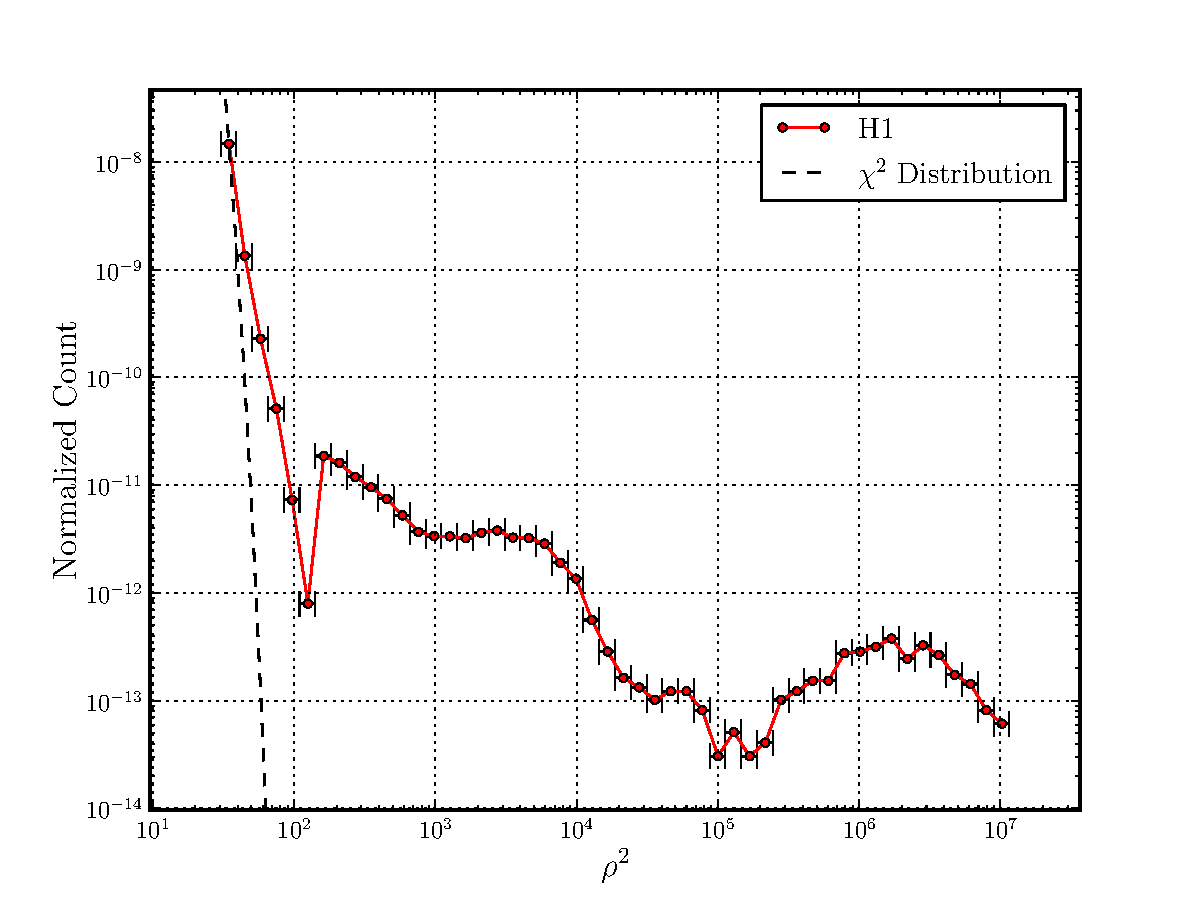
\includegraphics[width=6in]{figures/H1-snr_hist_cat1_veto.pdf}
\caption{Histogram of triggers as a function of SNR. Data is taken from two weeks of H1 data taken during S6. The mass range used for this plot is $\mtotal \in [2,25)\Msun$; see chapter \ref{ch:ihope_pipeline} for details on the templates used. This plot was created using a single-stage pipeline, as discussed in \ref{ch:future_developments}, rather than the two-stage pipeline discussed in \ref{ch:ihope_pipeline}. This was done so as to remove complications from the intermediate coincidence stage. A $\chi^2$ distribution with two degrees of freedom, expected if the detector output were Gaussian, is also plotted. Due to the SNR cutoff, it is difficult to determine the proper normalization. Here, we have normalized the data so that the bin with the largest count was made to lay on the $\chi^2$ distribution. In this case, the data was multiplied by $\sim10^{-14}$. The bin boundaries used are given by the x-error bars.}
\label{fig:snr_hist}
\end{figure}

\begin{figure}
\center
\subfigure[Non-spinning injections]{\label{fig:snr_chisq-nospin}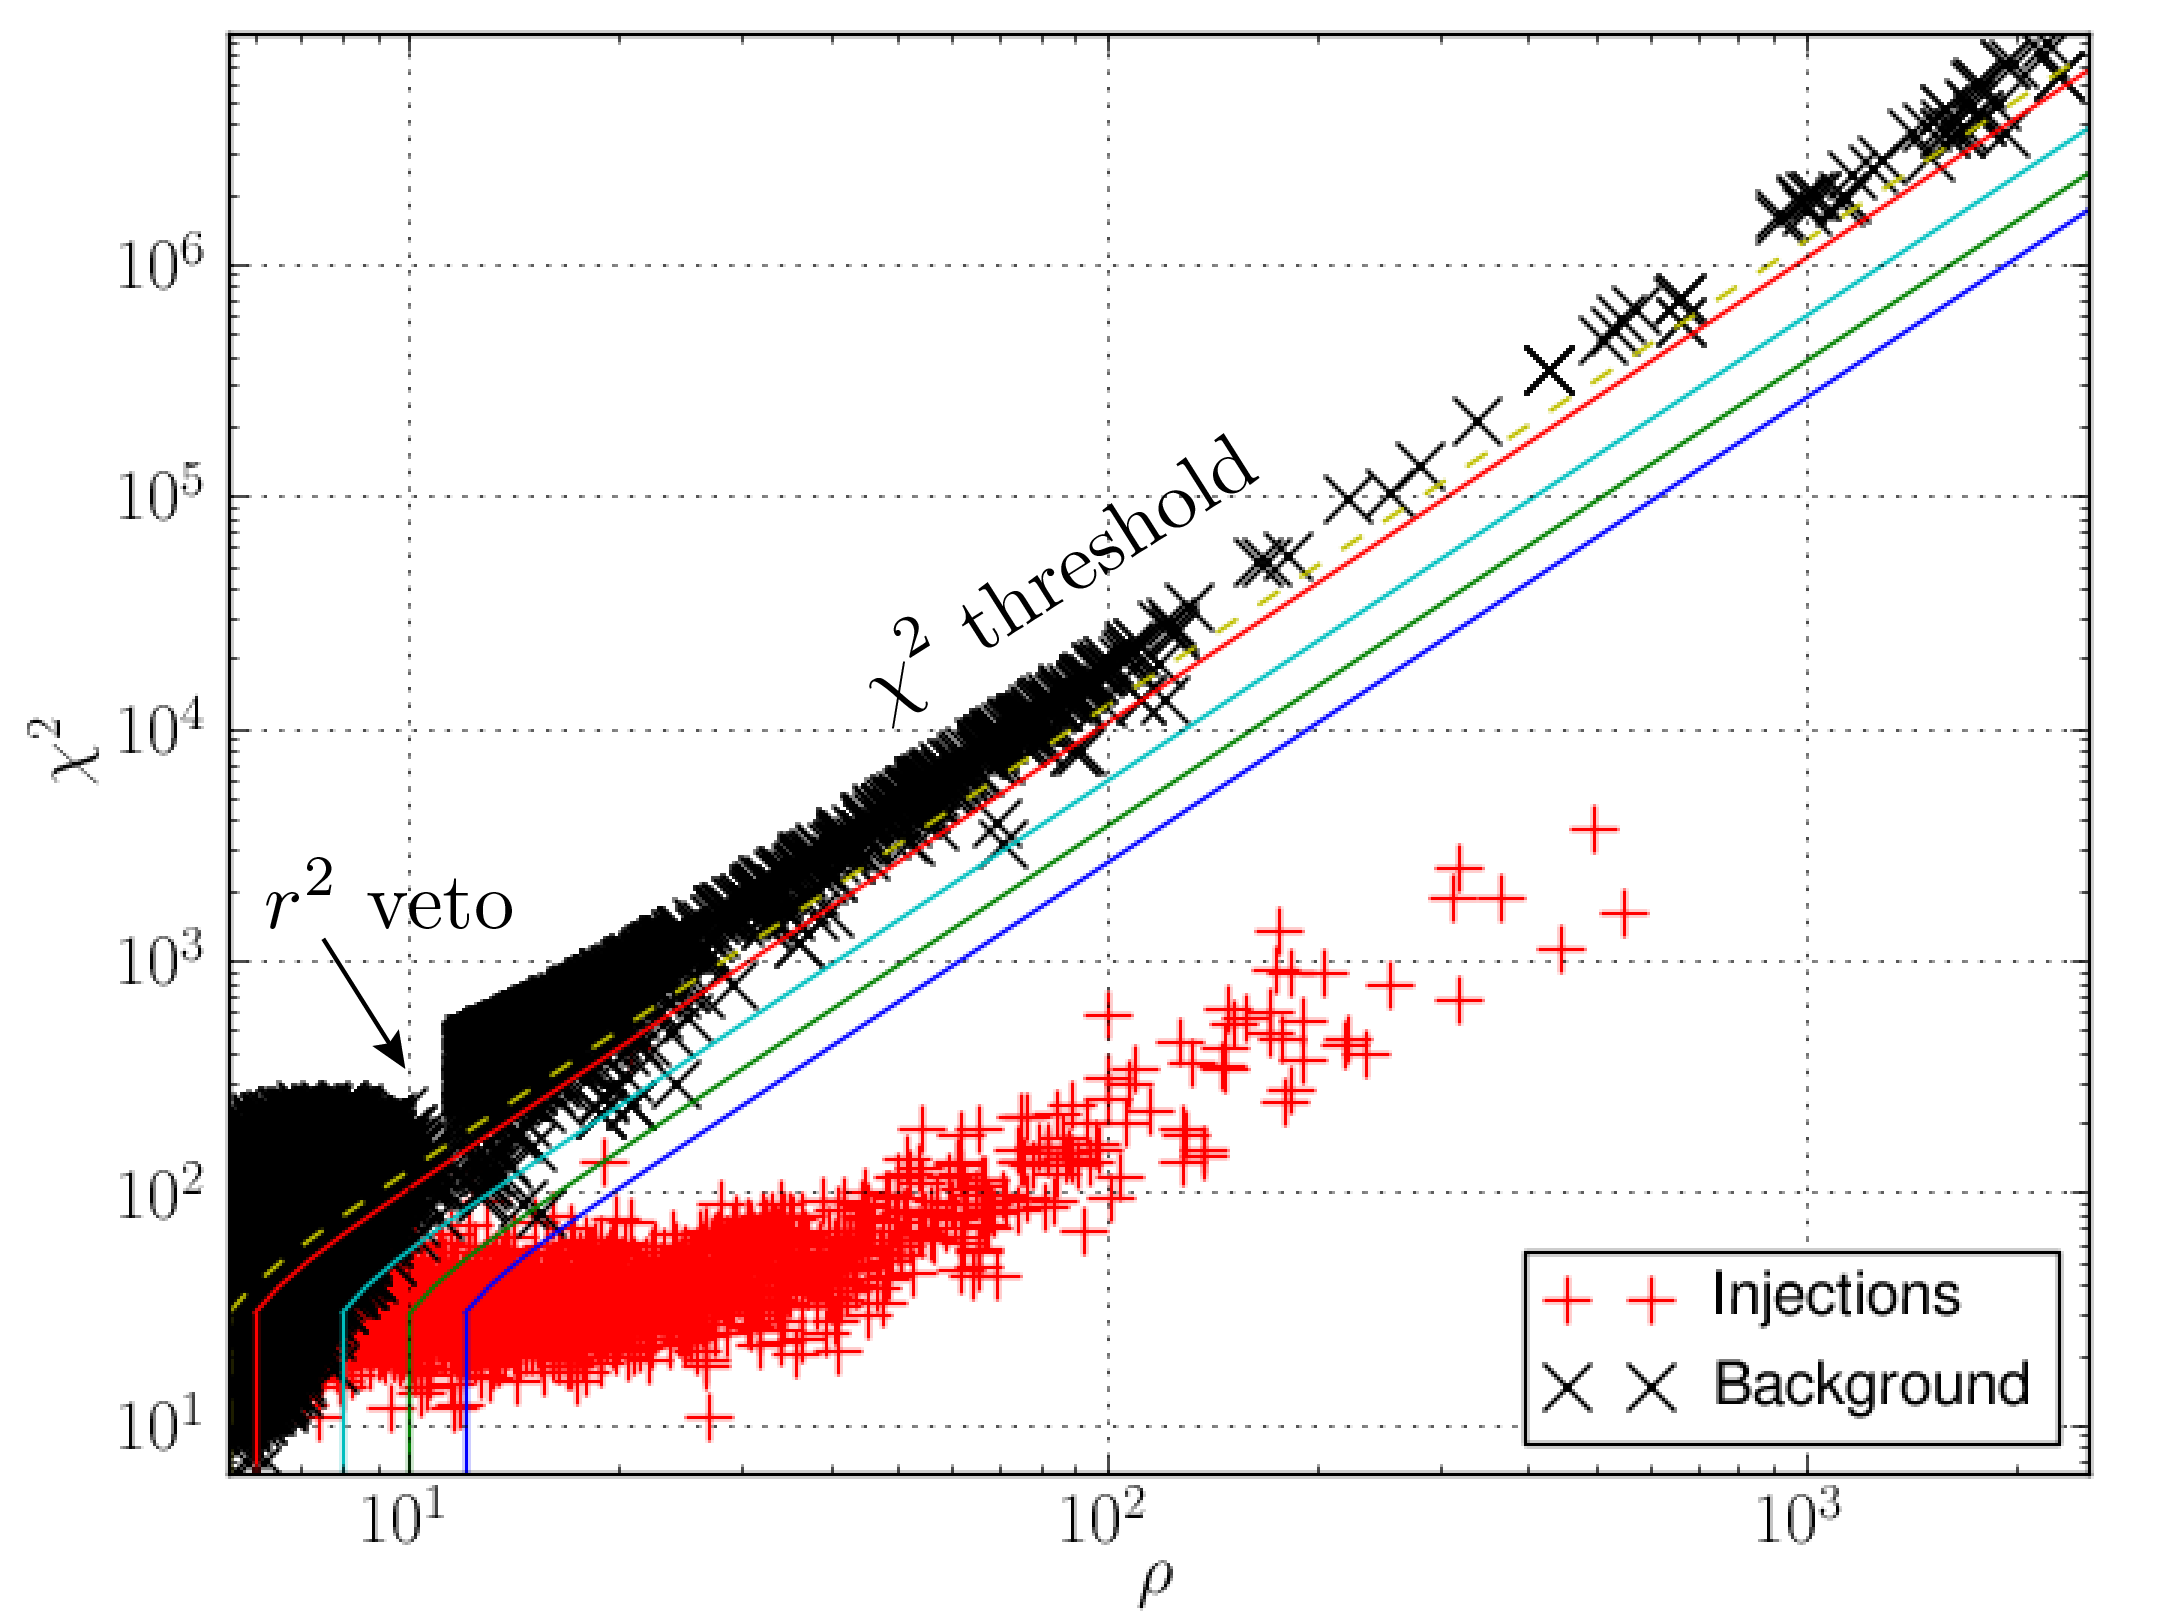
\includegraphics[width=4.5in]{figures/H1-plotsnrchi_nospin_cat1_snr_chisq-967593543-1209744.png}} \\
\subfigure[Spinning injections]{\label{fig:snr_chisq-spin}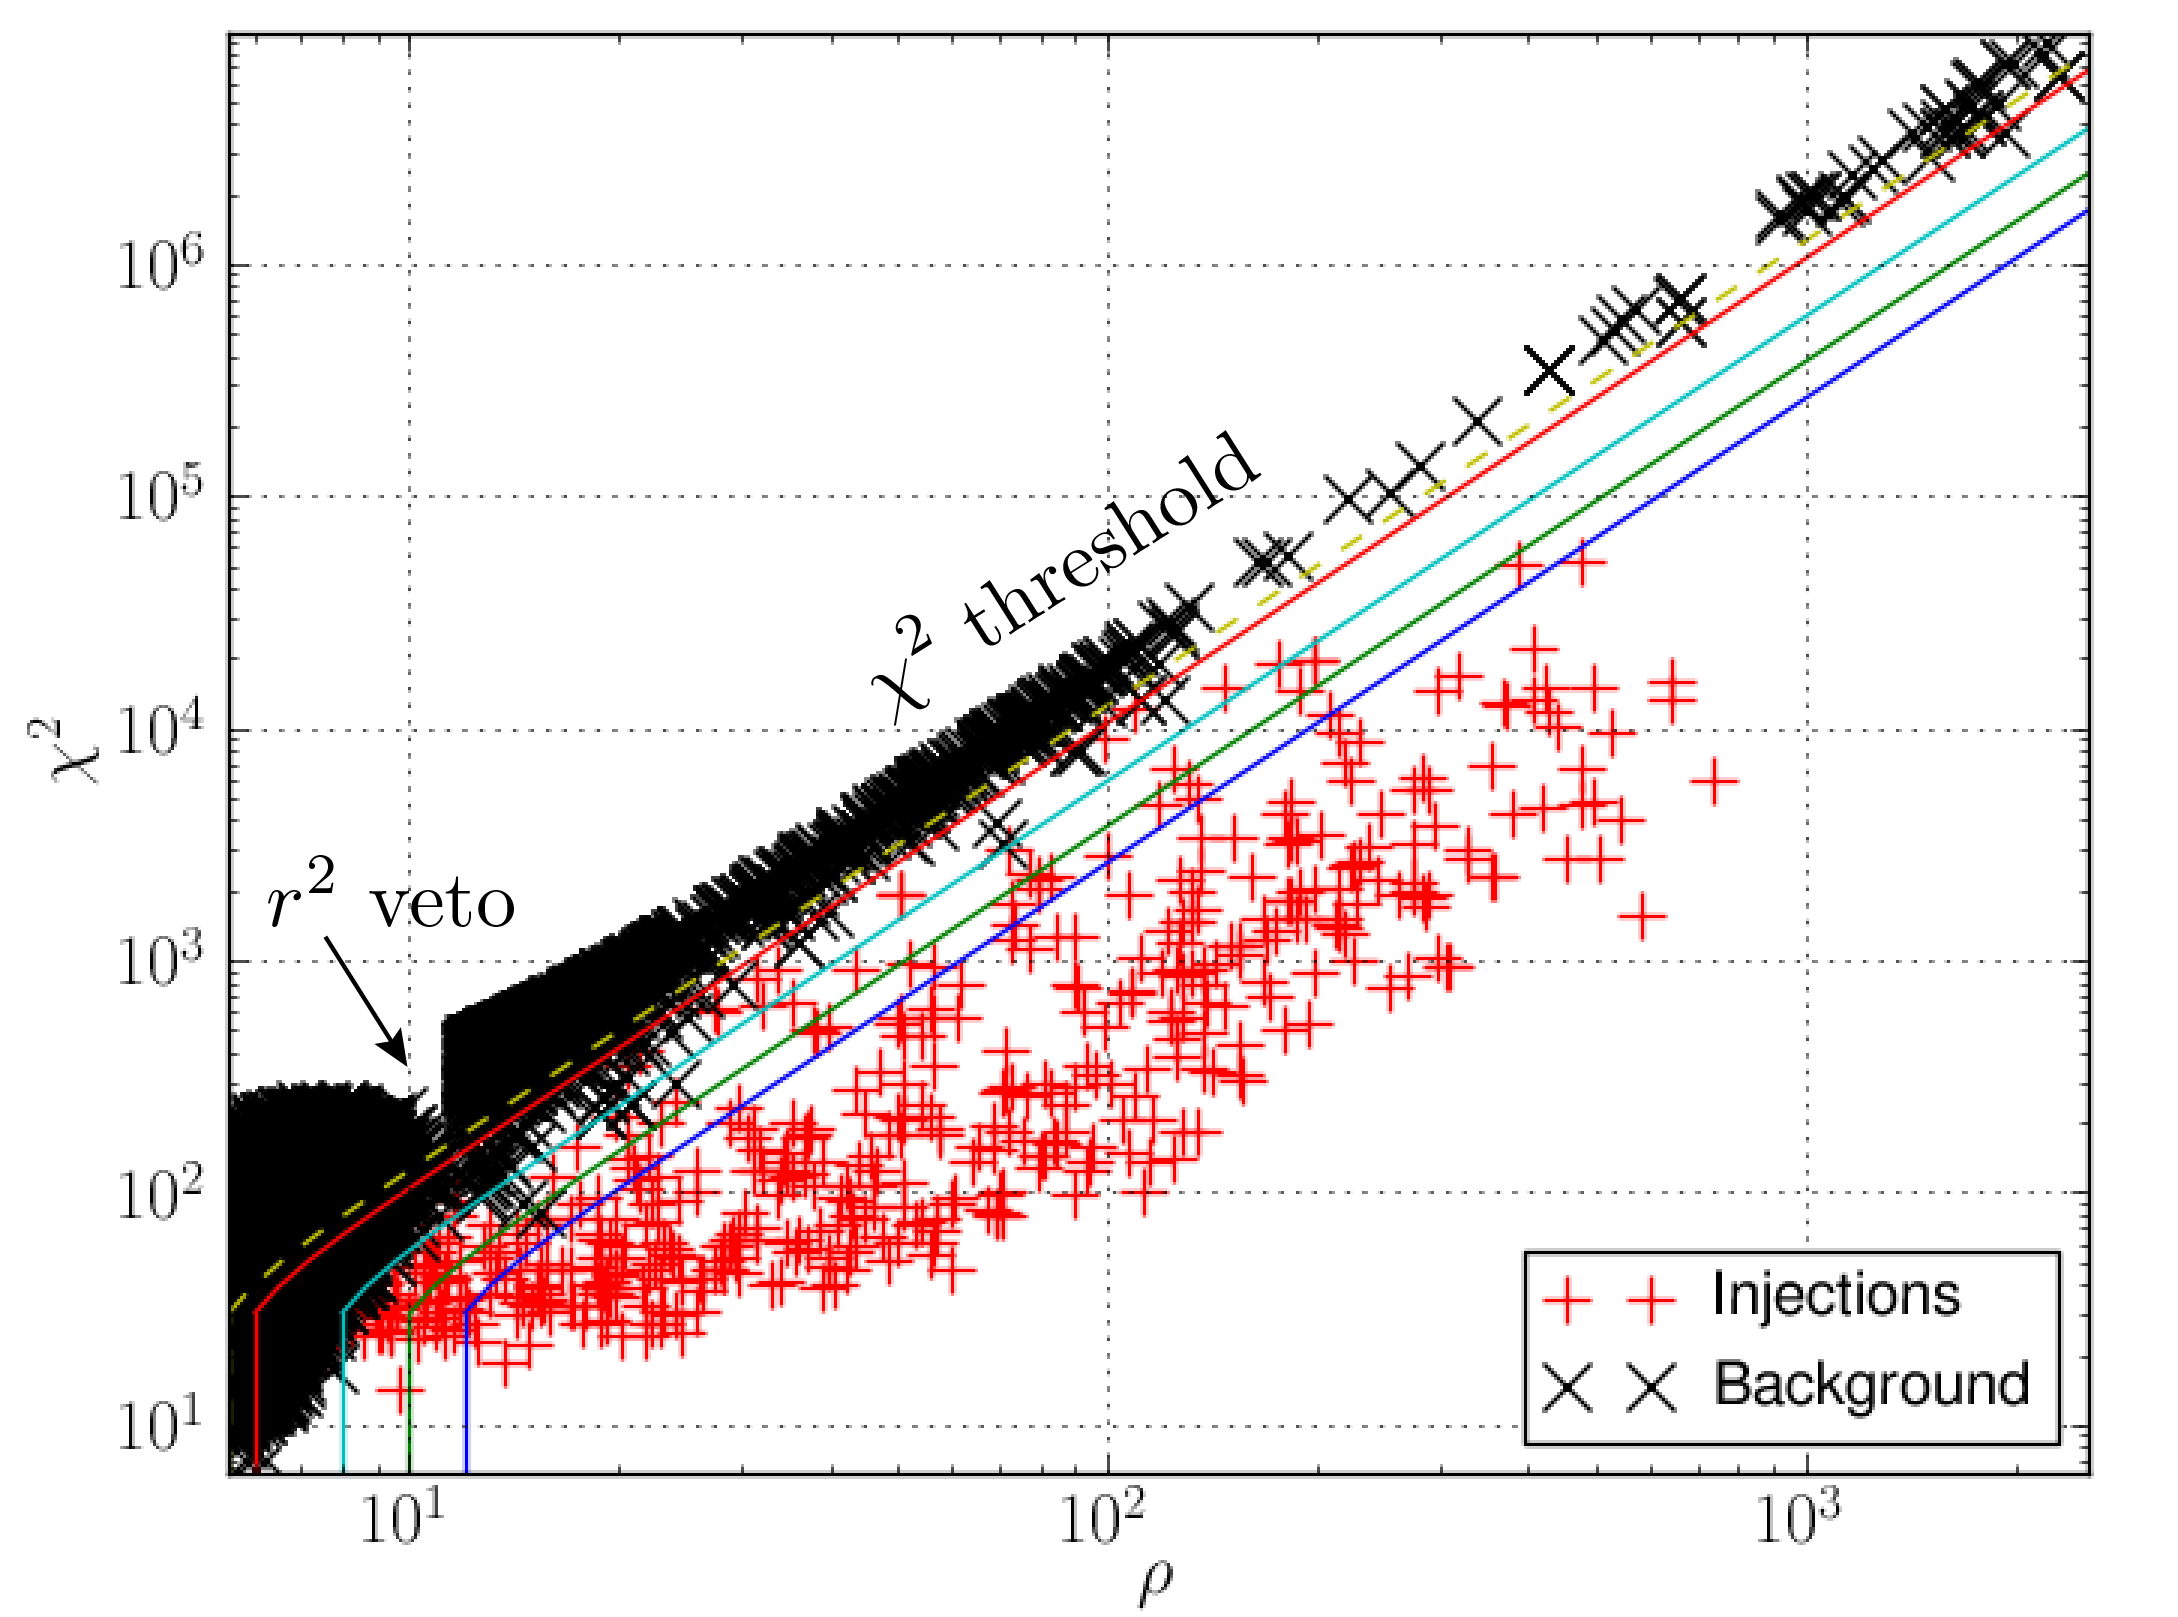
\includegraphics[width=4.5in]{figures/H1-plotsnrchi_spin_cat1_snr_chisq-967593543-1209744.png}}
\caption{$\chi^2$ versus SNR of H1 triggers taken from two weeks of S6. Black crosses indicate ``background" triggers, which are triggers that survived coincidence in time slides (see section \ref{sec:coincidence_test} and Chapter \ref{ch:far} for details). Red crosses indicate ``software injections" (see Chapter \ref{ch:ihope_pipeline} for details). Colored lines indicate points of constant New SNR. The effect of the $r^2$ veto and $\chi^2$ threshold are marked.}
\label{fig:snr_chisq}
\end{figure}

\begin{figure}
\center
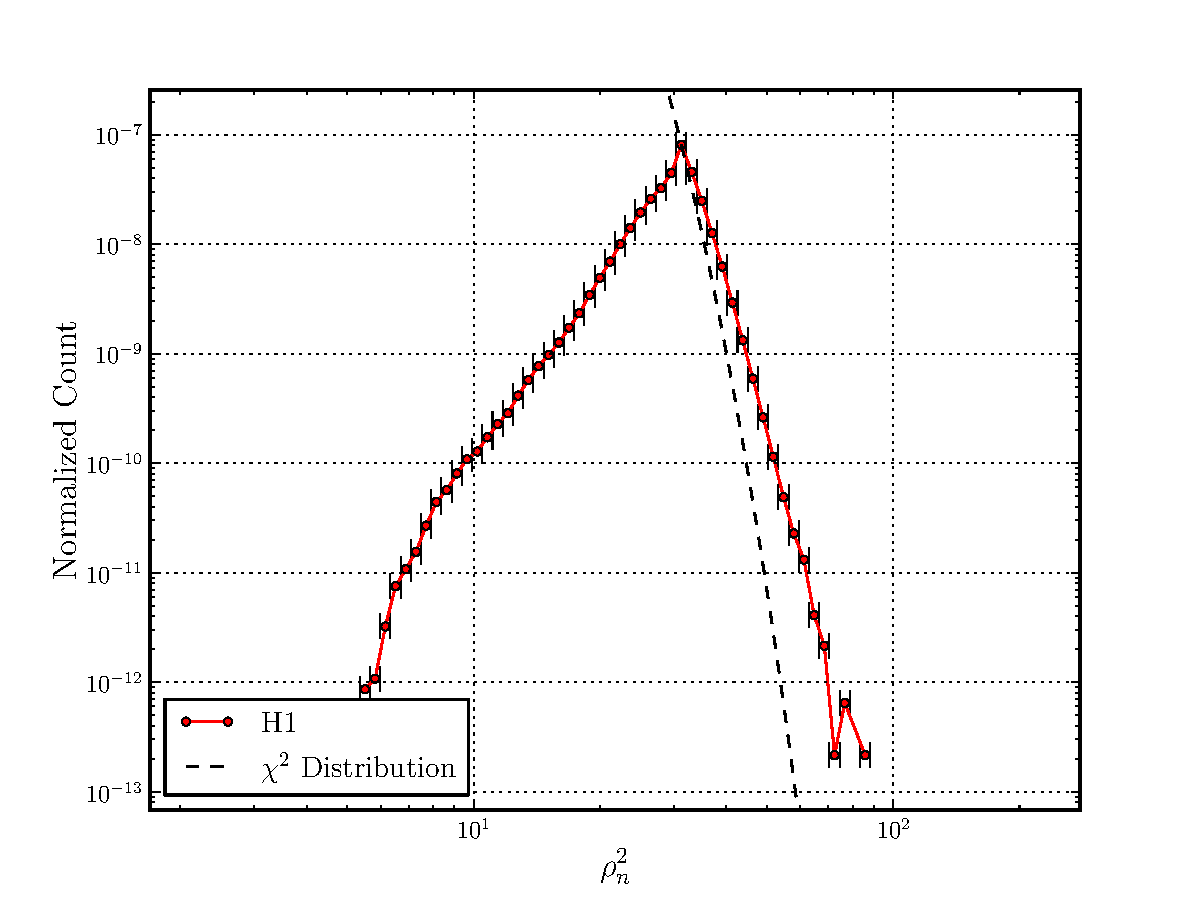
\includegraphics[width=6in]{figures/H1-newsnr_hist_cat1_veto.pdf}
\caption{Histogram of triggers as a function of New SNR. Data is the same as in \ref{fig:snr_hist}. A $\chi^2$ distribution with two degrees of freedom is plotted. As in Figure \ref{fig:newsnr_hist}, the normalization is chosen that the bin with the largest count lies along the distribution. In this case, the data was multiplied by $~10^{-13}$.}
\label{fig:newsnr_hist}
\end{figure}
